% --- Section 1: Présentation ---
\section{Contexte et objectifs}
\begin{frame}{Contexte et Objectifs}
        L'objectif de ce projet est de mettre en place un pipeline pour découvrir et évaluer des modèles de peptides \textit{in silico} en utilisant un enchaînement d'experts spécialisés sur certaines tâches.
        \\
        \minimize{in silico: réalisé par ordinateur, sans expérimentation physique.}
        \\
        \centering
        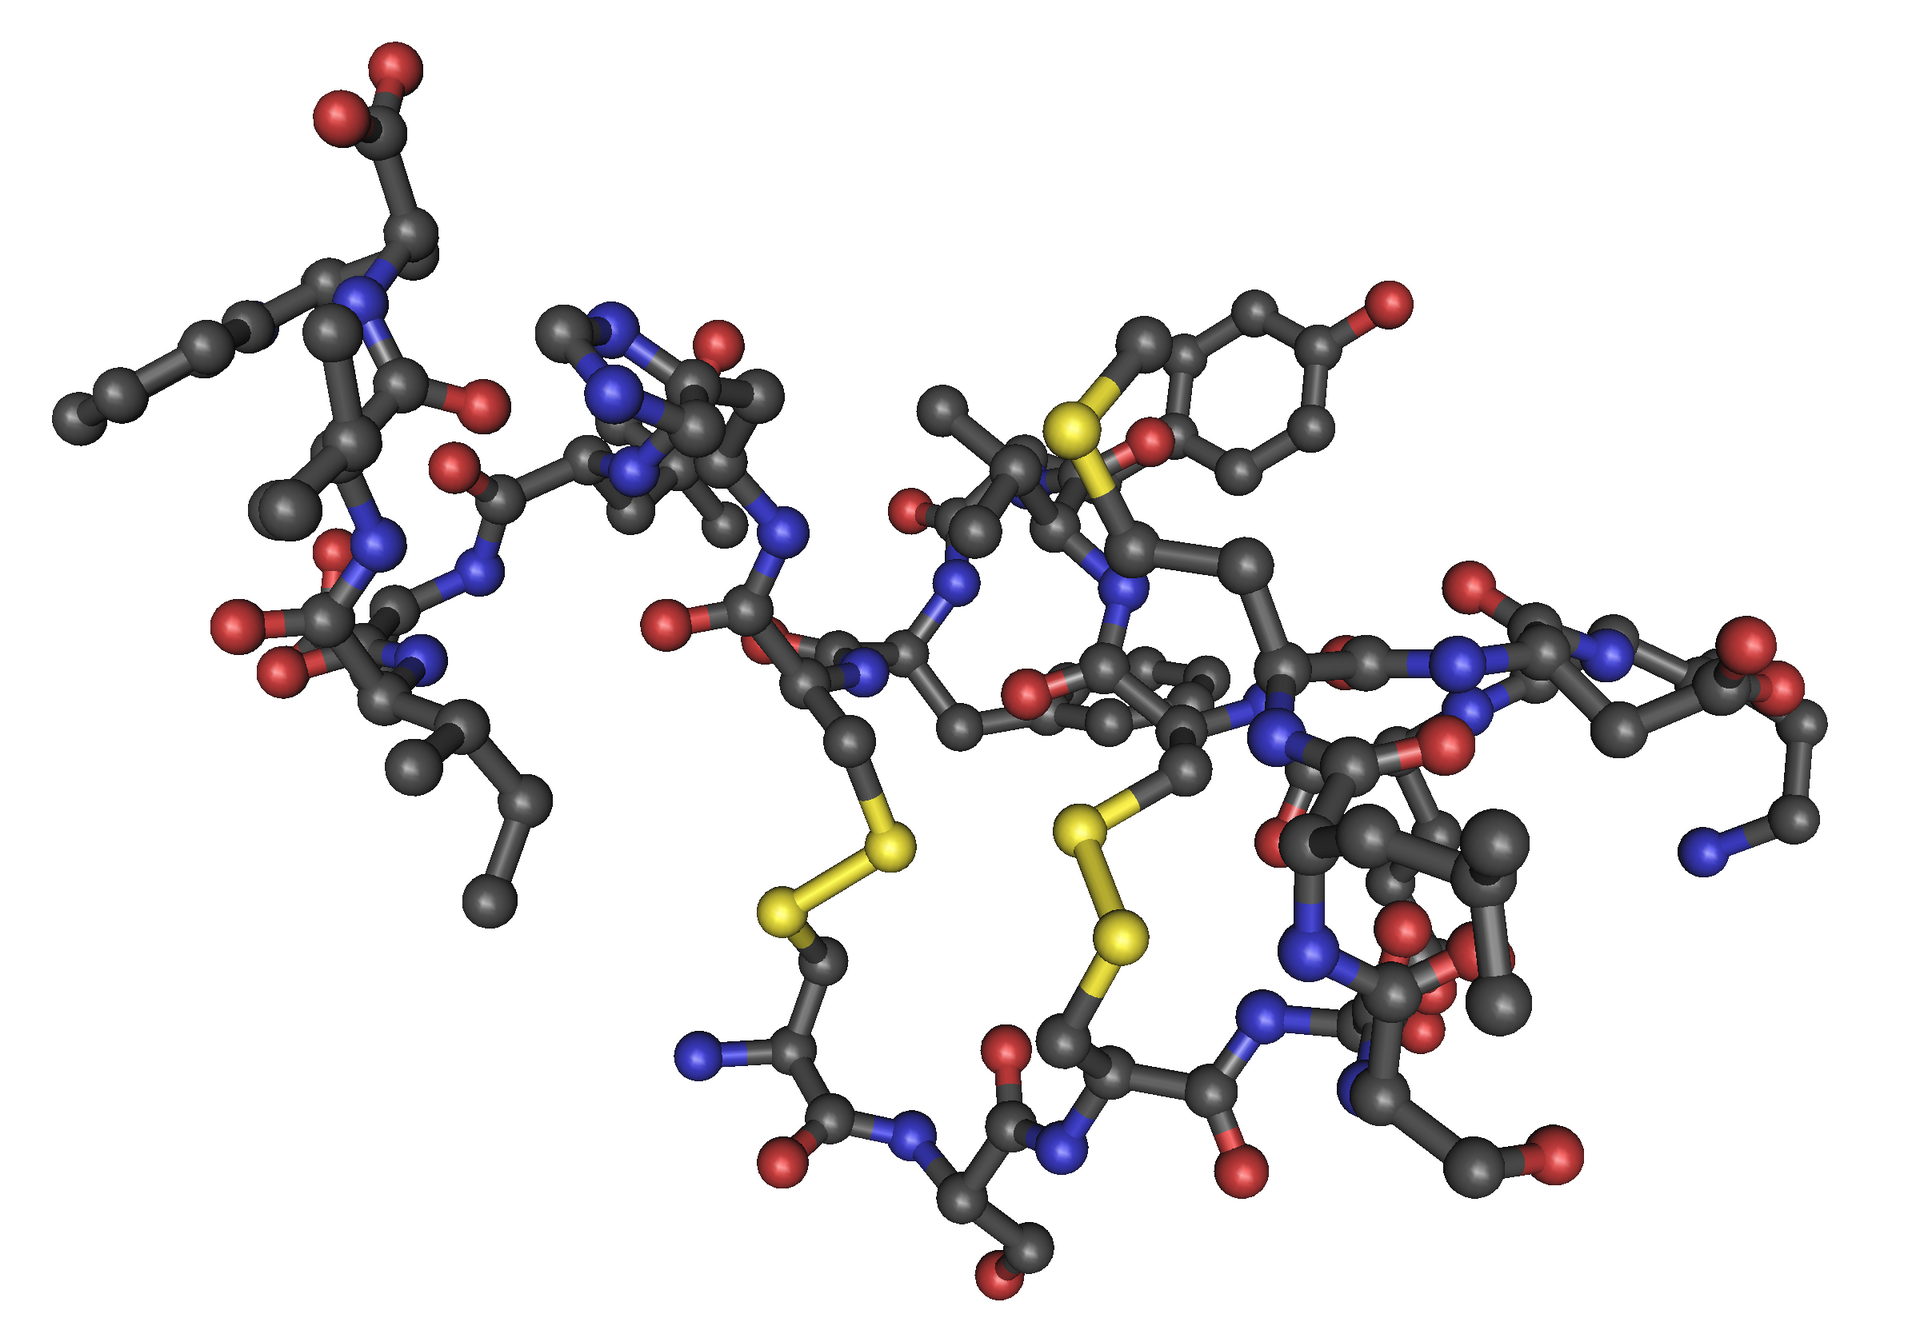
\includegraphics[height=4cm]{peptide.png}
\end{frame}

\begin{frame}
    \frametitle{Peptide}
    \begin{itemize}
        \item Chaîne composée d'au plus 50 acides aminés
        \item 20 acides aminés différents
        \item Applications: médecine, agriculture, industrie
        \item Exemples: insuline, antibiotiques, hormones
    \end{itemize}

    \begin{block}{Processus de découverte actuel}
        \begin{itemize}
            \item Découverte de peptides: criblage de bibliothèques, évolution dirigée
            \item Évaluation: tests biologiques, simulations moléculaires
            \item Itération sur les resultats pour améliorer l'efficacité de la peptides
            \item Coût élevé, temps long, taux de succès faible
        \end{itemize}
    \end{block}
\end{frame}